% !TeX program = xelatex
\documentclass[10pt,a4paper]{ctexart} % 设置文章类型，正文字号与纸张大小

% 页面与正文常用宏包
\usepackage[margin=2cm]{geometry} % 设置页面四周页边距
\usepackage{graphicx}             % 插入图片
\usepackage{amsmath}              % 提供cases、aligned等数学公式环境
\usepackage{amssymb}              % 提供\therefore等扩展数学符号
\usepackage{booktabs}             % 提供\toprule、\midrule、\bottomrule三线表命令
\usepackage{float}                % 提供[H]固定图片、表格位置
\usepackage{subcaption}           % 提供subfigure子图环境及子图标题
\usepackage{wrapfig}              % 提供wrapfigure图文环绕环境
\usepackage{fancyhdr}             % 自定义页眉和页脚
\usepackage{hyperref}             % 生成超链接

% 页眉页脚
\pagestyle{fancy}                  % 启用fancyhdr定义的页面样式
\fancyhf{}                         % 清空默认页眉和页脚
\fancyfoot[C]{\thepage}            % 在页脚中央显示页码
\renewcommand{\headrulewidth}{0pt} % 隐藏页眉横线
\renewcommand{\footrulewidth}{0pt} % 隐藏页脚横线

% 超链接
\hypersetup{
  colorlinks=true,                % 使用彩色文字链接，而非带边框的链接
  linkcolor=red,                 % 目录、公式及图表交叉引用的颜色
  filecolor=cyan,                 % 本地文件链接的颜色
  urlcolor=blue,                  % 网址链接的颜色
  pdftitle={分光计的调整和使用+棱镜偏向角特性预习报告},     % 写入PDF文档属性的标题
  bookmarksnumbered=true          % PDF书签显示章节编号
}

% 定义字号命令
\newcommand{\chuhao}{\fontsize{42pt}{63pt}\selectfont}
\newcommand{\xiaochu}{\fontsize{36pt}{54pt}\selectfont}
\newcommand{\yihao}{\fontsize{26pt}{39pt}\selectfont}
\newcommand{\xiaoyi}{\fontsize{24pt}{36pt}\selectfont}
\newcommand{\erhao}{\fontsize{22pt}{33pt}\selectfont}
\newcommand{\xiaoer}{\fontsize{18pt}{27pt}\selectfont}
\newcommand{\sanhao}{\fontsize{16pt}{24pt}\selectfont}
\newcommand{\xiaosan}{\fontsize{15pt}{22.5pt}\selectfont}
\newcommand{\sihao}{\fontsize{14pt}{21pt}\selectfont}
\newcommand{\xiaosi}{\fontsize{12pt}{18pt}\selectfont}
\newcommand{\wuhao}{\fontsize{10.5pt}{15.75pt}\selectfont}
\newcommand{\xiaowu}{\fontsize{9pt}{13.5pt}\selectfont}

% 章节格式
\ctexset{
  section={
    format={\CJKfontspec[AutoFakeBold=2.5]{KaiTi}\sanhao\bfseries}, % 一级标题使用三号加粗楷体
    name={,、},                                                    % 在中文章节序号后添加顿号
    number=\chinese{section},                                      % 一级标题编号使用“一、二、三”形式
    aftername={}                                                   % 取消编号与标题文字之间的空格
  },
  subsection={
    format={\CJKfontspec[AutoFakeBold=2.5]{KaiTi}\sihao\bfseries}, % 二级标题使用四号加粗楷体
  },
  subsubsection={
    format={\CJKfontspec[AutoFakeBold=2.5]{KaiTi}\xiaosi\bfseries}, % 三级标题使用小四加粗楷体
  }
}

\begin{document}

% 封面
\thispagestyle{fancy} % 封面保留底部居中的页码
\fancyfoot[C]{\thepage}
\begin{center}
  \CJKfontspec[AutoFakeBold=2.5]{KaiTi}\bfseries % 封面中文使用楷体并人工加粗，西文同时加粗
  \vspace*{2.0cm}
  \xiaochu 
    物理实验预习报告

  \vspace{3.8cm}
  \begin{minipage}{14.0cm}
    \sanhao
    \makebox[2.6cm][l]{实验名称：}
    \underline{\makebox[11.0cm][c]{分光计的调整和使用+棱镜偏向角特性}}\par\vspace{12pt}

    \makebox[2.6cm][l]{指导老师：}
    \underline{\makebox[11.0cm][c]{王兆英}}\par\vspace{12pt}
  \end{minipage}

  \vspace{3.8cm}
  \begin{minipage}{10.0cm}
    \sihao
    \makebox[1.4cm][l]{班级：}
    \underline{\makebox[8.0cm][c]{}}\par\vspace{10pt}

    \makebox[1.4cm][l]{姓名：}
    \underline{\makebox[8.0cm][c]{IllusoryRain}}\par\vspace{10pt}

    \makebox[1.4cm][l]{学号：}
    \underline{\makebox[8.0cm][c]{}}
  \end{minipage}

  \vspace{1.8cm}
  \sihao
    实验日期：
    \underline{\makebox[0.7cm][c]{2026}}年
    \underline{\makebox[0.7cm][c]{10}}月
    \underline{\makebox[1.4cm][c]{21/28}}日
    星期\underline{\makebox[1.4cm][c]{三/三}}上午

  \vspace{0.7cm}
  \sihao 
    浙江大学物理实验教学中心
\end{center}

\newpage
\xiaosi\songti\mdseries % 后续正文统一使用小四宋体

\section{预习报告（10分）}

  \subsection{实验综述（5分）}

    \subsubsection{分光计的调整和使用}
    分光计主要由平行光管、望远镜、载物台和读数装置组成。先目测预调，使望远镜、平行光管及载物台大致水平，再进行以下调整：
    \begin{enumerate}
      \item 调节目镜使叉丝清晰，利用双面平面镜进行自准直调节，使反射“十”字像清晰且与叉丝无视差。（可选）
      \item 调整叉丝方向，用“各半调节法”调节望远镜倾斜螺钉和载物台调平螺钉，使平面镜两面的反射像均与上方叉丝重合。
      \item 用望远镜观察平行光管狭缝，调节狭缝位置使像清晰且无视差，再调节光管倾斜及狭缝方向，使狭缝像竖直、居中且宽度适当。
    \end{enumerate}
    
    调整后，平行光管发出平行光，望远镜光轴、平行光管光轴及载物台平面均垂直于仪器主轴。

    本实验采用棱脊分束法测量三棱镜顶角。将待测顶角的棱脊朝向平行光管，
    平行光经构成顶角的两个光学面反射，形成夹角为顶角两倍的左、右两束反射光。
    保持载物台不动，用望远镜分别瞄准两侧反射狭缝像，记录两个位置的双游标读数，顶角为
    \[
    A=\frac{\left|\theta_{\text{右I}}-\theta_{\text{左I}}\right|
           +\left|\theta_{\text{右II}}-\theta_{\text{左II}}\right|}{4}
    \]
    
    其中，“左”“右”表示两侧反射像的位置，I、II表示两个游标。
    读数跨越零刻度时，应先作跨零处理；双游标读数取平均可减小刻度盘偏心引起的误差。

    这样操作是为了消除偏心差，此外读数也有一定要求，具体如下图：
    \begin{figure}[H]
      \centering
      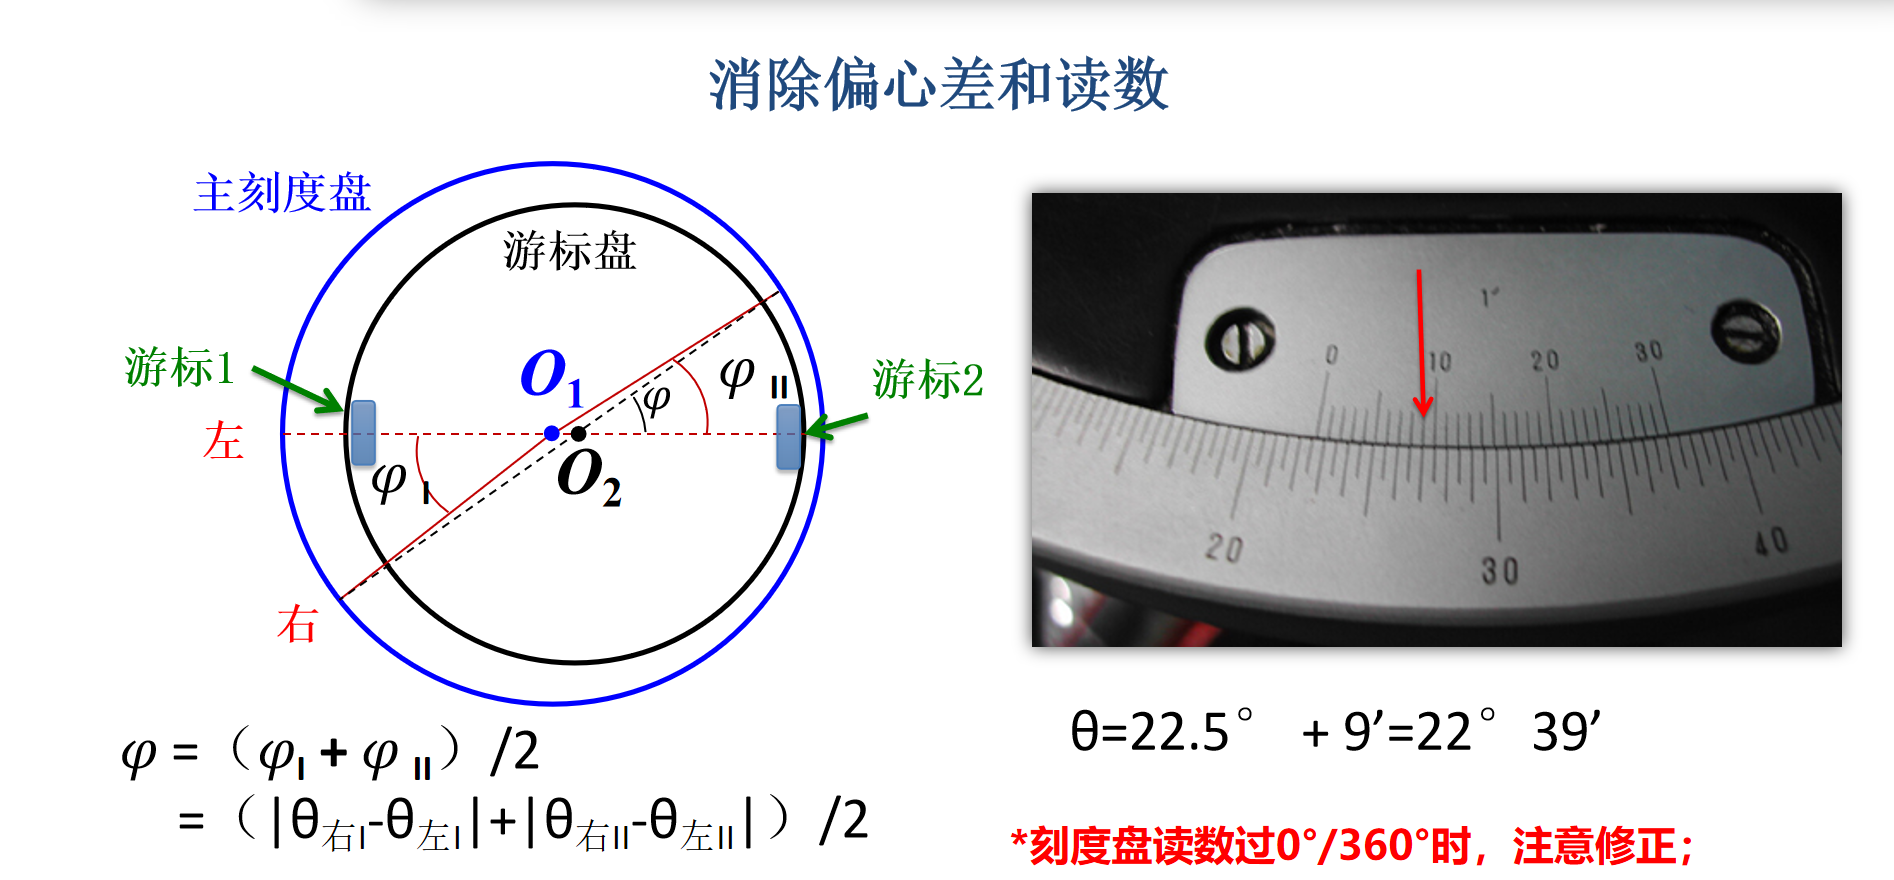
\includegraphics[width=0.65\textwidth]{figures/图1.png}
      \caption{消除偏心差和读数}
    \end{figure}

    综上本实验包括以下内容：
    \begin{enumerate}
      \item 了解分光计的结构。
      \item 用双面平面镜调整分光计。
      \item 用棱脊分束法测量三棱镜顶角。
    \end{enumerate}

    \subsubsection{棱镜偏向角特性}
    光线通过顶角为$A$、折射率为$n$的三棱镜时，由折射定律和几何关系可得
    \[
    \sin i_1=n\sin i_2 \qquad
    \sin i_4=n\sin i_3 \qquad
    i_2+i_3=A
    \]
    \[
    \delta=(i_1-i_2)+(i_4-i_3)=i_1+i_4-A
    \]
    
    其中，$i_1$、$i_4$分别为入射角和出射角，$i_2$、$i_3$为棱镜内的折射角和入射角。

    偏向角$\delta$随入射角增大先减小后增大。令$\dfrac{d\delta}{di_1}=0$，得
    $\dfrac{di_4}{di_1}=-1$；结合折射定律的微分关系及$di_2=-di_3$，可得
    \[
    \frac{\cos i_2}{\cos i_1}=\frac{\cos i_3}{\cos i_4}
    \]
    
    代入折射定律并化简，得$i_2=i_3$，从而$i_1=i_4$。
    此时光路对称，偏向角达到最小值，且
    \[
    i_2=i_3=\frac{A}{2} \qquad
    i_1=i_4=\frac{A+\delta_{\min}}{2}
    \]
    
    因此，测得顶角$A$和最小偏向角$\delta_{\min}$后，即可计算折射率：
    \[
    n=\frac{\sin\left(\dfrac{A+\delta_{\min}}{2}\right)}
           {\sin\left(\dfrac{A}{2}\right)}
    \]

    出射面$AC$的全反射临界角为$C=\arcsin(1/n)$。
    当$A=60^\circ$、$n\approx1.66$时，$C\approx37^\circ$，
    对应$i_2=A-C\approx23^\circ$、$i_1\approx40^\circ$；
    入射角低于该临界值时，光线在$AC$面发生全反射。

    \begin{figure}[H]
      \centering
      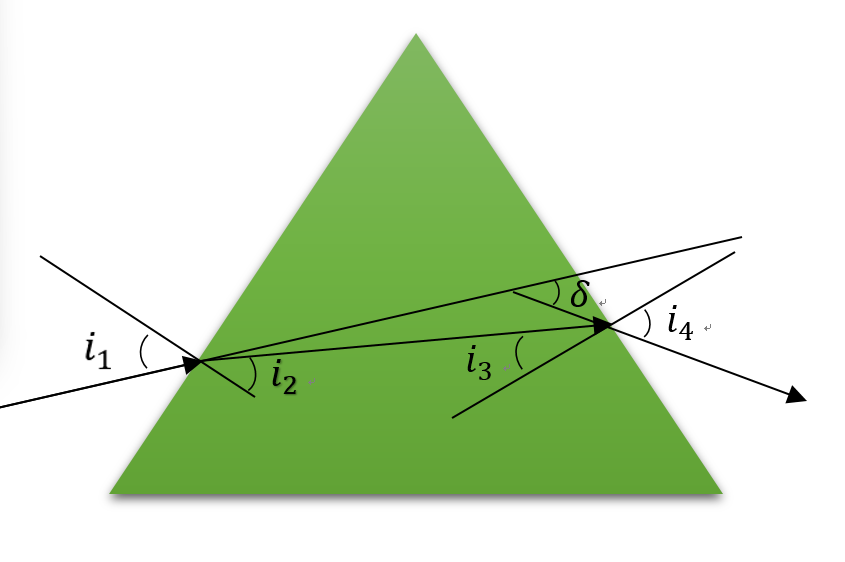
\includegraphics[width=0.4\textwidth]{figures/图2.png}
      \caption{最小偏向角测量原理图}
    \end{figure}

    实验包括以下内容：
    \begin{enumerate}
      \item 调整分光计
      \item 测量三棱镜顶角$A$
      \item 测量最小偏向角$\delta_{\min}$
      \item 计算三棱镜单色光折射率
      \item 绘制色散曲线并思考
    \end{enumerate}

  \subsection{实验重点（3分）}
  
    \subsubsection{分光计的调整和使用}
    \begin{enumerate}
      \item 了解分光计结构、光路和各部分作用
      \item 熟悉示波器面板旋钮的功能，掌握示波器的调节和使用方法。掌握分光计调整和使用
      \item 利用棱脊分束法测量三棱镜顶角
    \end{enumerate}

    \subsubsection{棱镜偏向角特性}
    \begin{enumerate}
      \item 分光计调整和使用
      \item 三棱镜顶角的测量
      \item 测量棱镜的折射率并研究其色散规律
    \end{enumerate}

  \subsection{实验难点（2分）}

    \subsubsection{分光计的调整和使用}
    \begin{enumerate}
      \item 利用双面平面镜调整望远镜与载物台，并调节平行光管，使其出射平行光。
      \item 准确辨认反射像和掠入射位置，正确读取双游标示数并计算角度。
      \item 正确辨认汞灯谱线及衍射级次，准确测量衍射角并计算波长。
    \end{enumerate}

    \subsubsection{棱镜偏向角特性}
    \begin{enumerate}
      \item 合理放置三棱镜，准确瞄准两面的反射像并测量顶角。
      \item 跟踪折射谱线，准确判断其转向位置并测量最小偏向角。
      \item 将各谱线波长与测量数据对应，计算折射率并分析色散曲线。
    \end{enumerate}

\vspace*{\fill} % 使下面内容在页面底部显示
\noindent
\begin{minipage}{\textwidth}
  注意事项：

  \begingroup
    \setlength{\leftskip}{2em} % 1--4整体向右缩进两个汉字宽度
    1. 用PDF格式上传“实验报告”，文件名：学生姓名+学号+实验名称+周次。

    2. “实验报告”必须递交在“学在浙大”本课程内对应实验项目的“作业”模块内。

    3. “实验报告”成绩必须在“浙江大学物理实验教学中心网站”-“选课系统”内查询。

    4. 教学评价必须在“浙江大学物理实验教学中心网站”-“选课系统”内进行，学生必须进行教学评价，才能看到实验报告成绩，教学评价须在本次实验结束之后3天内进行。\par
  \endgroup

  \begin{center}
    {\CJKfontspec[AutoFakeBold=2.5]{SimSun}\bfseries 浙江大学物理实验教学中心制}
  \end{center}
\end{minipage}

\end{document}


